\documentclass[compress,xcolor=table]{beamer}

% Packages
\usepackage[french]{babel}
\usepackage[utf8]{inputenc}
\usepackage[T1]{fontenc}
\usepackage{datetime}
\usepackage{fourier}
\usepackage{graphicx}
\usepackage{subcaption}
\usepackage{multirow}
\usepackage{booktabs}
\usepackage{csquotes}

% Possible options of the package (add/remove below in \usetheme call):
%  - nosectionpages: no pages between sections
%  - flama: use flama font, requires xelatex/lualatex + the font to compile
%  - compressminiframes: put the heading list bullets indications pages on 1 line
\usetheme[compressminiframes]{sorbonne}
\setbeamerfont{caption}{size=\tiny}

% Title page
\title{PLDAC}
\foottitle{} % optional, printed at the bottom of the slides, by default same as title, can be useful to rewrite when title has a newline for example
\subtitle{Chants d'oiseaux} % optional subtitle
\date{\formatdate{25}{05}{2023}}
\author{Valentin \textsc{Bencheci}, Aymeric \textsc{Delefosse}}
\institute{Master DAC - Sorbonne Université} % Optional

% Biblatex
\usepackage[backend=bibtex, style=authoryear, citestyle=authoryear]{biblatex}
\bibliography{library.bib}
\renewcommand*{\bibfont}{\footnotesize}


%%%%
%% BEGIN OF SLIDES
%%%%

\begin{document}

\begin{frame}[plain]
    \titlepage
    \setcounter{framenumber}{0}
\end{frame}


\section{DCASE} \subsection{}

\begin{frame}{Contexte}

    \begin{block}{Detection and Classification of Acoustic Scenes and Events}

        \begin{itemize}
            \item
                  Workshop \& Challenge annuels : rassemblement de la communauté de chercheurs du domaine du traitement du signal audio .
            \item
                  Se concentre principalement sur la détection et la classification des scènes et événements acoustiques.
        \end{itemize}

    \end{block}

    \begin{exampleblock}{Exemples}
        \begin{itemize}
            \item
                  2022 \& 2023 : \textit{Few-shot Bioacoustic Event Detection}
            \item
                  2021 : \textit{Automated Audio Captioning}
            \item
                  2018 : \textit{Bird audio detection} $\leftarrow$ notre problématique
        \end{itemize}
    \end{exampleblock}

\end{frame}

\begin{frame}{Quel lien avec DAC ?}

    Qui dit détection ou classification... implique souvent des techniques issues de l'apprentissage automatique.

    \begin{alertblock}{Mais...}
        La communauté du traitement du signal audio a connu un certain décalage par rapport aux développements dans les domaines de l'informatique et de la data science.
    \end{alertblock}

    \begin{block}{Pourquoi ?}
        \begin{itemize}
            \item Complexité et de la spécificité des données audio.
            \item Communauté qui a évolué de manière relativement isolée $\Rightarrow$ manque de transfert de connaissances.
        \end{itemize}

    \end{block}

\end{frame}

\begin{frame}{Quel lien avec DAC ?}

    Mais depuis ces dernières années, il existe une convergence plus étroite entre les deux communautés.

    \begin{exampleblock}{Les données au c\oe ur de tout}
        \begin{itemize}
            \item Avancées dans le \textit{deep learning} dans ce domaine, grâce aux réseaux de neurones convolutionnels et récurrents.
            \item Soutenues par la disponibilité de grandes quantités de données audio.
            \item Progrès de l'informatique distribuée.
        \end{itemize}
    \end{exampleblock}

\end{frame}

\section{Challenge et données} \subsection{}

\begin{frame}{\textit{Bird Audio Detection}}

    \begin{block}{Challenge}
        \begin{itemize}
            \item Développer un système capable de détecter la présence ou l'absence de sons d'oiseaux dans des enregistrements audio.
            \item Décision binaire ou probabiliste $\in [0,1]$.
            \item $\Rightarrow$ Capacité à généraliser (défi important).
        \end{itemize}
    \end{block}

\end{frame}

\begin{frame}{Données}

    \begin{block}{Freefield}
        \begin{itemize}
            \item Enregistrements de terrain à travers le monde.
            \item Diversité des emplacements et des environnements.
            \item \warning Classes déséquilibrées : 25~\% sons d'oiseaux
        \end{itemize}
    \end{block}

    \begin{block}{Warblr}
        \begin{itemize}
            \item Enregistrements audio provenant d'utilisateurs de l'application Warblr, couverture variée des emplacements et des environnements britanniques.
            \item Bruits de fond tels que le trafic, les voix humaines et les imitations d'oiseaux par les humains.
            \item \warning Classes déséquilibrées : 75~\% sons d'oiseaux
        \end{itemize}
    \end{block}

\end{frame}

\begin{frame}{Données}

    \begin{block}{BirdVox}
        \begin{itemize}
            \item Enregistrements effectués par des unités de surveillance à distance.
            \item Échantillonnage uniforme sur différents moments de la journée et conditions météorologiques.
            \item Classes équilibrées
        \end{itemize}
    \end{block}

    Au total : 35~690 enregistrements avec 17~997 sons contenant des chants d'oiseaux et 17~693 sons n'en contenant pas.

\end{frame}

\begin{frame}{Principal défi}

    \begin{figure}[ht]
        \centering
        \begin{subfigure}[b]{0.45\textwidth}
            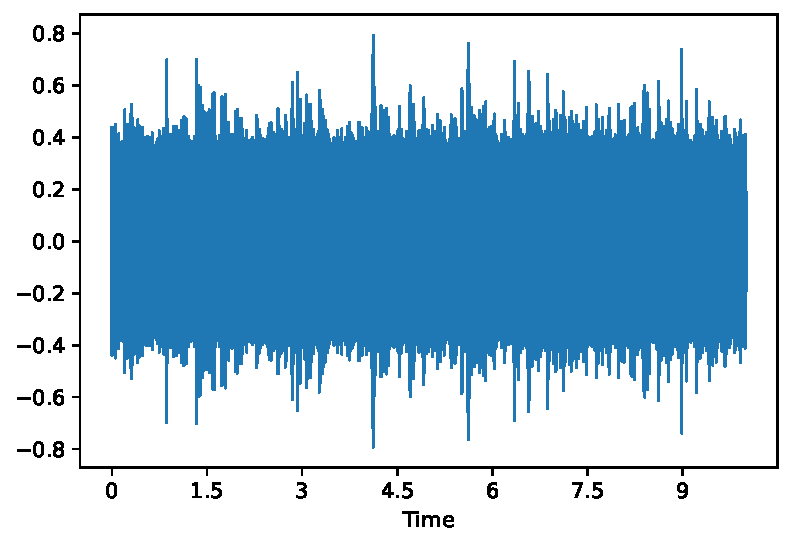
\includegraphics[width=\textwidth]{images/audio/birds.wave.birdvox.pdf}
            \caption{Enregistrement contenant des oiseaux}
            \label{fig:birds.wave.birdvox}
        \end{subfigure}
        \hfill
        \begin{subfigure}[b]{0.45\textwidth}
            \centering
            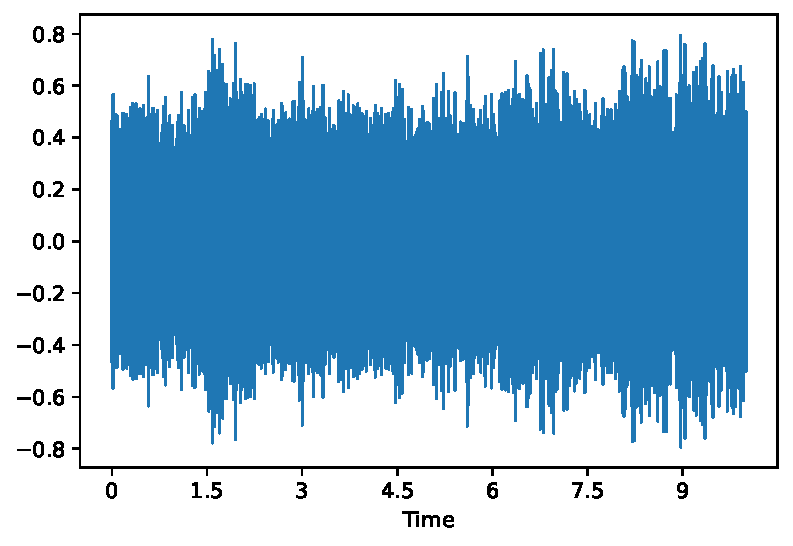
\includegraphics[width=\textwidth]{images/audio/nobirds.wave.birdvox.pdf}
            \caption{Enregistrement ne contenant pas d'oiseaux}
            \label{fig:nobirds.wave.birdvox}
        \end{subfigure}

        \vspace{-0.5cm}

        \begin{subfigure}[b]{0.45\textwidth}
            \centering
            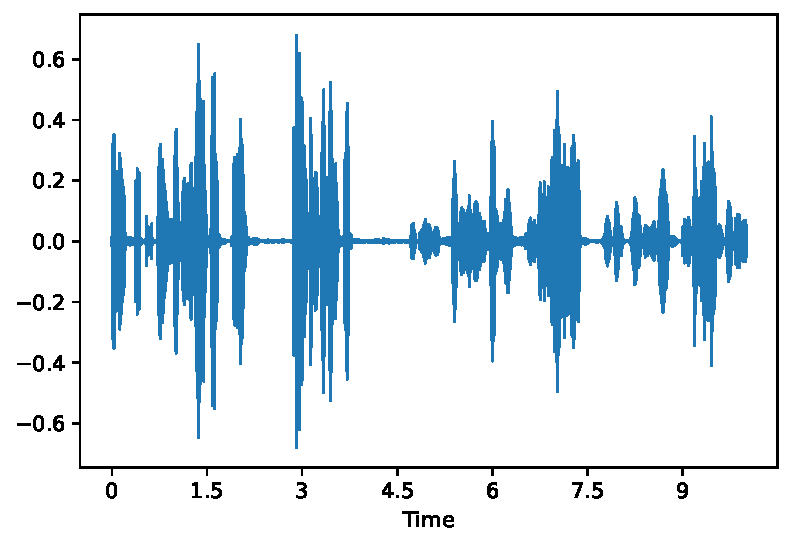
\includegraphics[width=\textwidth]{images/audio/birds.wave.ff1010.pdf}
            \label{fig:birds.wave.ff1010}
        \end{subfigure}
        \hfill
        \begin{subfigure}[b]{0.45\textwidth}
            \centering
            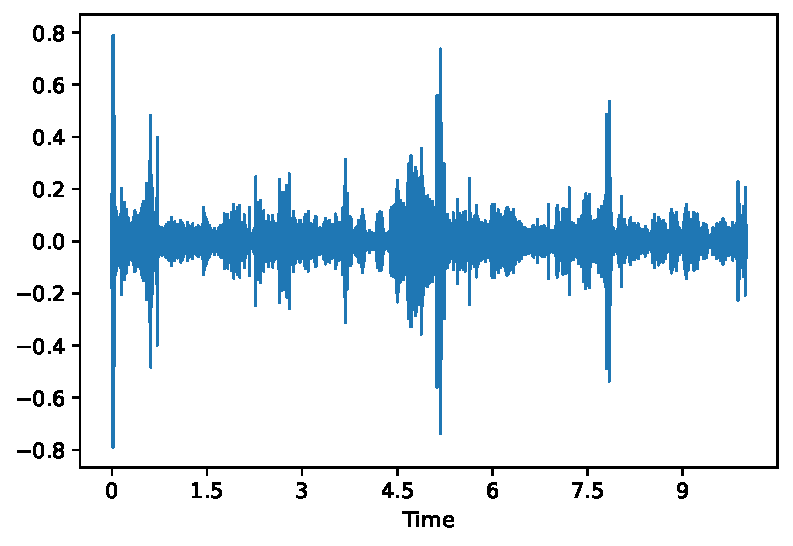
\includegraphics[width=\textwidth]{images/audio/nobirds.wave.ff1010.pdf}
            \label{fig:nobirds.wave.ff1010}
        \end{subfigure}
    \end{figure}

\end{frame}

\begin{frame}{Représentation temporelle (forme d'onde)}

    \begin{block}{Avantages}
        \begin{itemize}
            \item Visualiser intuitive du signal audio. % permettant de détecter les changements rapides ou lents dans l'amplitude du son.
            \item Identifier les moments de silence ou de faible amplitude, ainsi que les pics et les moments d'intensité sonore élevée.
            \item Repérer des motifs ou des caractéristiques spécifiques dans le signal audio.
        \end{itemize}
    \end{block}

    \begin{alertblock}{Inconvénients}
        \begin{itemize}
            \item Pas d'informations détaillées sur la nature exacte des composantes fréquentielles du son.
            \item Ne permet pas d'identifier précisément les différentes sources sonores présentes dans le signal.
            \item Limité par la résolution temporelle de l'affichage. % ce qui peut rendre difficile la détection de variations très rapides ou de détails fins dans le signal audio.
        \end{itemize}
    \end{alertblock}

\end{frame}

\begin{frame}{Représentation spectrale}
    Nécessité de se tourner vers des représentations \textbf{spectrales}.

    \begin{block}{Avantages}
        \begin{itemize}
            \item Visualiser des composantes fréquentielles du signal audio. % permettant de détecter les changements rapides ou lents dans l'amplitude du son.
            \item Identifier les changements de fréquence, les harmoniques et les caractéristiques spectrales spécifiques.
            \item Utile pour la \textbf{détection d'événements sonores}, la classification d'instruments, l'analyse musicale...
        \end{itemize}
    \end{block}

    \begin{alertblock}{Inconvénients}
        \begin{itemize}
            % \item Pas d'informations détaillées sur les variations temporelles du signal audio.
            \item Peut nécessiter une résolution temporelle plus fine pour représenter les variations rapides dans le signal.
            \item Processus parfois irréversible...
        \end{itemize}
    \end{alertblock}

\end{frame}

\begin{frame}{Représentation spectrale}
    Mais il existe plusieurs représentations... laquelle choisir ?

    \begin{exampleblock}{Les plus communes...}
        \begin{itemize}
            \item Spectrogramme ?
            \item Chromagramme ?
            \item Cepstre ?
        \end{itemize}
    \end{exampleblock}

    $\Rightarrow$ Dans tous les cas : Fourier !
\end{frame}

\begin{frame}{Représentation spectrale : Chromagramme}
    

    \begin{figure}[ht]
        \centering
        \begin{subfigure}[b]{0.45\textwidth}
            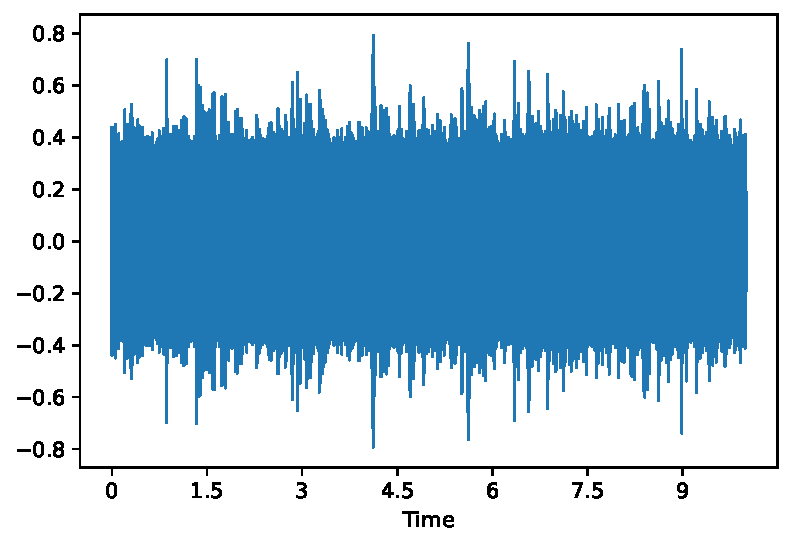
\includegraphics[width=\textwidth]{images/audio/birds.wave.birdvox.pdf}
            \caption{Enregistrement contenant des oiseaux}
            \label{fig:1}
        \end{subfigure}
        \hfill
        \begin{subfigure}[b]{0.45\textwidth}
            \centering
            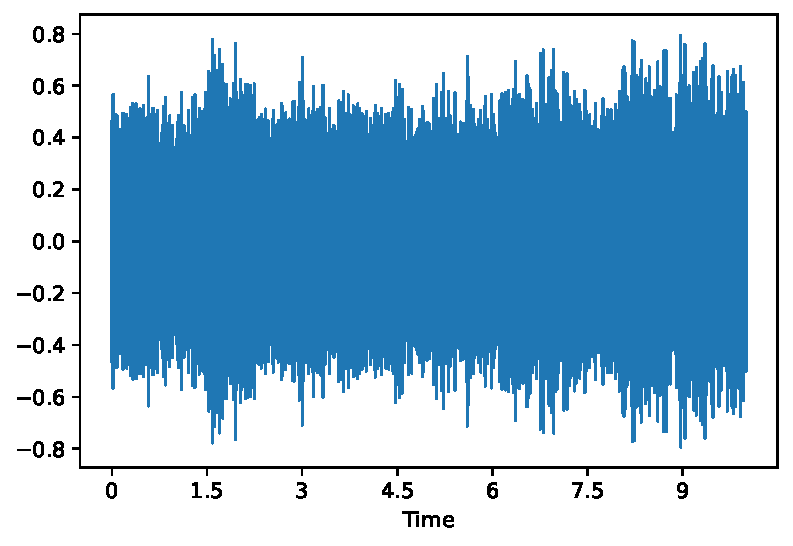
\includegraphics[width=\textwidth]{images/audio/nobirds.wave.birdvox.pdf}
            \caption{Enregistrement ne contenant pas d'oiseaux}
            \label{fig:2}
        \end{subfigure}
    \end{figure}
    

\end{frame}

\begin{frame}{Représentation spectrale : Chromagramme}
    Mais il existe plusieurs représentations... laquelle choisir ?

    \begin{block}{Chromagramme}

        \begin{itemize}
            \item Représentation temps/notes de musique.
            \item Met l'accent sur les informations tonales et harmoniques d'un signal audio.
            \item Largement utilisé dans des applications telles que la transcription musicale automatique, la reconnaissance des accords et l'analyse comparative de morceaux de musique.
        \end{itemize}

    \end{block}

    $\Rightarrow$ Représentation \textbf{non pertinente} pour notre problème.

\end{frame}

\begin{frame}{Représentation spectrale : Spectrogramme}
    Mais il existe plusieurs représentations... laquelle choisir ?

    \begin{block}{Spectrogramme}

        \begin{itemize}
            \item Représentation temps/fréquence.
            \item Met l'accent sur la répartition spectrale de l'énergie ou de la puissance du signal audio.
            \item Utile pour observer les changements de fréquences, les harmoniques, les transitions tonales et les événements sonores dans le temps.
            \item Possibilité de passer en 3D : temps/fréquence/amplitude.
        \end{itemize}

    \end{block}

    $\Rightarrow$ Représentation \textbf{pertinente} pour notre problème.

\end{frame}


\begin{frame}{Représentation spectrale : Cepstre}
    Mais il existe plusieurs représentations... laquelle choisir ?

    \begin{block}{Cepstre}
        
        \begin{itemize}
            \item Met l'accent sur l'étude structures périodiques temporelles des caractéristiques spectrales d'un signal audio.
            \item Fournit des informations sur les enveloppes spectrales et les variations dans le domaine fréquentiel du signal.
            \item Utile pour l'analyse des formants vocaux, la détection des harmoniques, la reconnaissance de la parole et d'autres applications liées aux caractéristiques temporelles du signal audio.
            \item Réversible !
        \end{itemize}

    \end{block}

    $\Rightarrow$ Représentation \textbf{pertinente} pour notre problème.

\end{frame}

\section{Expérimentations et résultats} \subsection{}

\begin{frame}{Performance}

    \begin{table}[h]
        \centering
        \resizebox{\linewidth}{!}{
            \begin{tabular}{llcccccc}
                \toprule
                \multirow{2}{*}{Modèle}                 & \multirow{2}{*}{Pooling} & \multicolumn{2}{c}{Freefield1010} & \multicolumn{2}{c}{Warblrb10K} & \multicolumn{2}{c}{BirdVox}                                                 \\
                                                        &                          & AUC                               & F1                             & AUC                         & F1            & AUC           & F1            \\
                \midrule
                $\textrm{CNN}$                          & Max probability          & .847                              & .730                           & .849                        & .926          & .873          & .860          \\
                $\textrm{CNN}$                          & Temporal                 & .842                              & .706                           & .853                        & \textbf{.937} & .888          & \textbf{.885} \\
                \midrule
                $\textrm{CRNN}_{RNN}$                   & Temporal                 & .841                              & .708                           & .789                        & .921          & .877          & .868          \\
                \midrule
                $\textrm{CRNN}_{LSTM}$                  & Temporal                 & .857                              & .783                           & .868                        & .906          & .882          & .873          \\
                $\textrm{CRNN}_{LSTM}$                  & Soft Attention           & .849                              & .783                           & .858                        & .908          & .870          & .857          \\
                \midrule
                $\textrm{CRNN}_{\textit{Transformers}}$ & Temporal                 & .820                              & .755                           & .844                        & 884           & .836          & .811          \\
                \midrule
                $\textrm{CRNN}_{GRU}$                   & Max probability          & \textbf{.861}                     & .778                           & .860                        & .908          & .882          & .872          \\
                $\textrm{CRNN}_{GRU}$                   & Temporal                 & .840                              & .719                           & .818                        & .923          & .890          & .883          \\
                $\textrm{CRNN}_{GRU}$                   & Soft Attention           & .859                              & \textbf{.784}                  & \textbf{.870}               & .916          & \textbf{.891} & .883          \\
                \bottomrule
            \end{tabular}
        }
        \caption{Performance de différents modèles sur Freefield, Warblr et BirdVox}
        \label{tab:performance}
    \end{table}

\end{frame}

\begin{frame}{Some papers for noisy images datasets}

    \begin{exampleblock}{\citetitle{cakirConvolutionalRecurrentNeural2017a} \cite{cakirConvolutionalRecurrentNeural2017a}}

        \begin{itemize}
            \item
                  Define a regularized loss for training the CNN
            \item
                  Can be seen as looking for the label of similar images for
                  regularization
            \item
                  Results slightly better than Sukhbaatar model
        \end{itemize}

    \end{exampleblock}

\end{frame}

\section{References} \subsection{}

\begin{frame}[allowframebreaks]{References}

    \printbibliography[heading=none]

\end{frame}




\end{document}

